Tal y como ocurría en el modelo SIS, los contactos entre poblaciones se van a representar con el producto de variables y los factores $\alpha I$ y $\beta SI$ serán equivalentes respectivamente, a la recuperación de un porcentaje $\alpha$ de individuos infectados y al paso al estado de infección por parte de un porcentaje $\beta$ de individuos susceptibles, luego de tener contacto con infectados\cite{diego2010}.

\section*{Autómatas celulares}
Son un modelo matemático capaz de describir el comportamiento de diferentes sistemas dinámicos, están compuestos por un conjunto de agentes (también llamados celdas, células, individuos o píxeles) que toman algún valor o estado.

El \textit{estado} de cada individuo es alterado en mediciones discretas de tiempo, usualmente esta alteración del estado de la célula depende del comportamiento sus individuos cercanos también llamados \textit{vecinos}, la regla que describe la relación entre el conjunto de estados, el agente y sus vecinos está determinada por una expresión matemática la cual se conoce la \textit{regla de evolución local}.\cite{descripcionyAplicaciones}

Para definir las reglas de evolución local de manera que se tengan en cuenta las tasas de infección y de recuperación, junto con el estado de cada vecino se usarán las reglas semi-totalísticas, las cuales consideran el estado de la célula central para posteriormente asignar un elemento del conjunto de estados a la suma de los valores de los elementos que forman la vecindad, estos valores determinan el comportamiento de todas las vecindades cuya suma de valores de sus elementos corresponda a un mismo valor.\cite{ACaplicacionesComputacion}

Cada individuo puede tomar un único valor del conjunto de estados que se modelan con el autómata celular, en nuestro caso será uno de dos estados para el modelo SIS (o tres en el caso del modelo SIR). Es importante resaltar la complejidad que puede llegar a tener un autómata celular, debido al comportamiento en la vecindad de cada celda.

En el caso de sistemas 2-dimensionales encontramos una gran cantidad de vecindades, entre las más conocidas encontramos la \textit{vecindad de Von Neumann} la cual considera a la célula central y a los individuos ubicados a la izquierda, derecha, arriba y abajo y la \textit{vecindad de Moore} la cual añade los individuos diagonales a la vecindad de Von Neumann. Para los intereses del proyecto, se decidió trabajar con vecindades de Moore. 

\begin{center}
	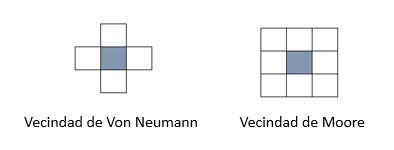
\includegraphics[width=0.5\textwidth]{Imagenes/vecindades.PNG}
\end{center}
\begin{center}
    \caption{Fuente: Jorge Ibañez 2021}
\end{center}

Aunque si bien, la investigación iniciará sobre las redes regulares definidas sobre las vecindades de Von Neumann y las vecindades de Moore, lo ideal es implementar diferentes tipos de vecindad que permitan fortalecer los aspectos predictivos del algoritmo en redes neuronales. Para esto será necesario tener presentes algunas nociones de topologías definidas a partir de vecindades.

\section*{Topología}
Durante esta sección se mencionan algunos de los conceptos relacionados con topología que se usaran durante el desarrollo del proyecto. Uno de los objetivos del proyecto es analizar el impacto de los cambios de topología, para lo cual debemos tener presentes los conceptos de topología definida por un sistema de vecindades, familias de vecindades entre otros. Se desarrolló una recopilación de definiciones extraídas de \cite{filtrosTopologia,munkres,elementosTopologiaGeneral}.